\documentclass{article}
\usepackage{graphicx}
\usepackage{float}
\usepackage{listings}
\usepackage{xcolor}
\usepackage{hyperref}
\usepackage{caption}

\lstset{
    basicstyle=\ttfamily\small,
    breaklines=true,
    frame=single,
    columns=fullflexible
}

\renewcommand{\lstlistingname}{Listado}
\renewcommand{\figurename}{Figura}

\title{Proyecto de análisis de datos SQL: Optimización de las decisiones de recursos humanos}
\author{Diego Armando Mijares Ledezma A01722421 \and Daniel Eduardo Arana Bodart A01741202 \and Mauricio Octavio Valencia Gonzalez A01234397 \and David Alejandro Acuña Orozco A00571187 \and Diego Gutiérrez Vargas A01285421 \and Alfonso Elizondo Partida A01285151}
\date{Mayo 23 2026}

\begin{document}

\maketitle
\tableofcontents
\newpage

%%%%%%%%%%%%%%%%%%%%%%%%%%%%%%%%%%%%%%%%%%%%%
\section{Resumen Ejecutivo}
%%%%%%%%%%%%%%%%%%%%%%%%%%%%%%%%%%%%%%%%%%%%%

Este análisis tuvo como objetivo comprender la composición, estabilidad, movilidad y compensación de la fuerza laboral de la empresa a partir de la base de datos \texttt{employees}, tomando como fecha de referencia el \textbf{31 de diciembre de 2002} cuando fue necesario. En términos generales, los resultados muestran una organización de gran escala, con \textbf{300024 empleados registrados}, una fuerza laboral madura, con una \textbf{edad promedio de 43.92 años}, y una estructura demográfica en la que no existe un equilibrio total de género, ya que \textbf{59.99\%} de la plantilla corresponde a hombres y \textbf{40.01\%} a mujeres. Estos hallazgos permiten dimensionar la magnitud de la operación y ofrecen una primera visión sobre la composición del talento humano dentro de la empresa.

Asimismo, el análisis evidencia una organización con una dinámica importante de crecimiento interno y estabilidad laboral. Se identificó que \textbf{140270 empleados} han ocupado más de un cargo, lo que sugiere una práctica extendida de movilidad interna, mientras que quienes cambian de puesto permanecen en su primer rol un promedio de \textbf{6.79 años}. A esto se suma una \textbf{antigüedad promedio de 12.92 años} entre los empleados activos, lo que apunta a una fuerza laboral estable y con experiencia acumulada. Por otro lado, las contrataciones muestran una tendencia descendente a lo largo del tiempo después de un periodo inicial de fuerte expansión, sin patrones estacionales especialmente marcados por mes o día de la semana. Finalmente, en materia de compensación, se observó un \textbf{salario promedio de 71964.80} al cierre de 2002, acompañado de una evolución salarial ascendente a lo largo de los años y de diferencias relevantes entre departamentos y puestos. En conjunto, estos resultados ofrecen a Recursos Humanos una base sólida para fortalecer estrategias de planeación de talento, diversidad e inclusión, desarrollo profesional, retención y revisión de estructuras de compensación.

\newpage

%%%%%%%%%%%%%%%%%%%%%%%%%%%%%%%%%%%%%%%%%%%%%
\section{Parte 1: Comprensión de la Fuerza Laboral}
%%%%%%%%%%%%%%%%%%%%%%%%%%%%%%%%%%%%%%%%%%%%%

\subsection{Demografía y Tamaño de la Fuerza Laboral}

\subsubsection{¿Cuántos empleados tenemos en total?}
\textbf{Necesidad de Negocio:} Recursos Humanos necesita rastrear el tamaño de la fuerza laboral para planificar recursos y contrataciones.

\textbf{SQL QUERY:}
\begin{lstlisting}[language=SQL, caption={Consulta -- Total de Empleados}]
SELECT 
    COUNT(DISTINCT emp_no) AS NumEmpleados
FROM employees.employees;
\end{lstlisting}

\textbf{Hallazgos:}

La consulta realizada sobre la tabla \texttt{employees} muestra que la empresa cuenta con un total de \textbf{300024 empleados registrados}.

\textbf{Insights:}

El resultado evidencia que la organización opera con una fuerza laboral de gran escala, lo que implica una estructura compleja de gestión del talento humano. Para el área de Recursos Humanos, conocer que existen \textbf{300024 empleados} permite dimensionar con mayor claridad las necesidades de planeación, reclutamiento, administración salarial y distribución de personal. Además, este dato funciona como base para análisis posteriores relacionados con departamentos, puestos, antigüedad y compensaciones, ya que ofrece un panorama general del tamaño de la operación.

\begin{figure}[H]
\centering
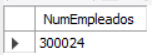
\includegraphics[width=0.3\textwidth]{imagenes/NumEmpleados.png}
\caption{Resultado -- Total de Empleados}
\end{figure}

\subsubsection{¿Cuál es la distribución de edad de nuestros empleados? (Mínimo, Máximo, Promedio)}
\textbf{Necesidad de Negocio:} Entender la estructura de edad e identificar los segmentos más jóvenes y experimentados de la fuerza laboral.

\textbf{SQL QUERY:}
\begin{lstlisting}[language=SQL, caption={Consulta -- Distribución de Edad de Empleados}]
SELECT
    MIN(TIMESTAMPDIFF(YEAR, birth_date, '2002-12-31')) AS EdadMinima,
    MAX(TIMESTAMPDIFF(YEAR, birth_date, '2002-12-31')) AS EdadMaxima,
    ROUND(AVG(TIMESTAMPDIFF(YEAR, birth_date, '2002-12-31')), 2) AS EdadPromedio
FROM employees.employees;
\end{lstlisting}

\textbf{Hallazgos:}

A partir de la consulta realizada, se identificó que, al 31 de diciembre de 2002, la \textbf{edad mínima} de los empleados es de \textbf{37 años}, la \textbf{edad máxima} es de \textbf{50 años} y la \textbf{edad promedio} es de \textbf{43.92 años}.

\textbf{Insights:}

Los resultados muestran que la fuerza laboral de la empresa se concentra en un rango de edad relativamente maduro, con un promedio cercano a los \textbf{44 años}. Esto sugiere una plantilla con experiencia laboral consolidada, lo cual puede representar ventajas en términos de conocimiento organizacional, estabilidad y especialización. Al mismo tiempo, este comportamiento demográfico puede ser relevante para Recursos Humanos al momento de diseñar estrategias de desarrollo, sucesión y renovación del talento, especialmente si se busca mantener un equilibrio generacional dentro de la organización.

\begin{figure}[H]
\centering
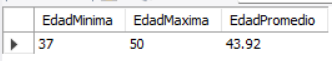
\includegraphics[width=0.5\textwidth]{imagenes/Edades.png}
\caption{Resultado -- Distribución de Edad de Empleados}
\end{figure}

\subsubsection{¿Existe equilibrio de género en nuestra fuerza laboral?}
\textbf{Necesidad de Negocio:} Medir la diversidad y asegurar la igualdad de oportunidades en la contratación.

\textbf{SQL QUERY:}
\begin{lstlisting}[language=SQL, caption={Consulta -- Distribución por Género}]
SELECT
    gender AS Genero,
    COUNT(*) AS NumEmpleados,
    ROUND(COUNT(*) * 100.0 / (SELECT COUNT(*) FROM employees.employees), 2) AS Porcentaje
FROM employees.employees
GROUP BY gender;
\end{lstlisting}

\textbf{Hallazgos:}

La consulta muestra que la fuerza laboral está compuesta por \textbf{179,973 empleados masculinos} y \textbf{120,051 empleadas femeninas}. En términos porcentuales, esto representa un \textbf{59.99\%} de hombres y un \textbf{40.01\%} de mujeres dentro del total de empleados registrados.

\textbf{Insights:}

Los resultados indican que \textbf{no existe un equilibrio de género completo} en la fuerza laboral, ya que la participación masculina es considerablemente mayor que la femenina. Desde una perspectiva de negocio, esta distribución puede señalar oportunidades para fortalecer estrategias de diversidad e inclusión, especialmente en los procesos de reclutamiento y selección. Para Recursos Humanos, este hallazgo es relevante porque permite identificar brechas en la composición demográfica de la empresa y puede servir como base para impulsar políticas que promuevan una representación más balanceada entre géneros.

\begin{figure}[H]
\centering
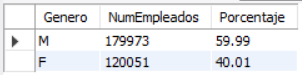
\includegraphics[width=0.5\textwidth]{imagenes/DistribucionGenero.png}
\caption{Resultado -- Distribución por Género}
\end{figure}

\subsubsection{¿Cuántos empleados han cambiado de departamento?}
\textbf{Necesidad de Negocio:} Identificar el nivel de movilidad interdepartamental y evaluar si la empresa promueve la rotación entre áreas.

\textbf{SQL QUERY:}
\begin{lstlisting}[language=SQL, caption={Consulta -- Empleados con Cambio de Departamento}]
SELECT COUNT(*) AS total_empleados_con_cambios
FROM (
    SELECT emp_no
    FROM dept_emp
    GROUP BY emp_no
    HAVING COUNT(DISTINCT dept_no) > 1
) AS empleados_movidos;
\end{lstlisting}

\textbf{Hallazgos:}

Los empleados que se movieron cambiaron a un máximo de \textbf{2 departamentos}. La movilidad interdepartamental existe pero es limitada, ya que ningún empleado registra haber pertenecido a más de dos departamentos distintos.

\textbf{Insights:}

La movilidad interdepartamental es baja. Esto puede indicar que los empleados se especializan en sus áreas o que hay pocas oportunidades de rotación interdepartamental. Desde la perspectiva de RH, impulsar programas de rotación entre áreas podría ampliar las habilidades del talento y fortalecer la colaboración entre departamentos.

\begin{figure}[H]
\centering
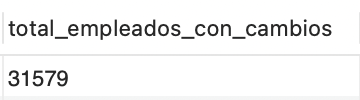
\includegraphics[width=0.5\textwidth]{imagenes/EmpleadosCambiaronDepartamento.png}
\caption{Resultado -- Empleados con Cambio de Departamento}
\end{figure}


\subsection{Crecimiento y Movilidad Interna}

\subsubsection{¿Cuántos empleados han tenido más de un cargo o puesto?}
\textbf{Necesidad de Negocio:} Identificar el volumen de movilidad interna y promociones.

\textbf{SQL QUERY:}
\begin{lstlisting}[language=SQL, caption={Consulta -- Empleados con Más de un Cargo}]
SELECT
    COUNT(*) AS EmpleadosConMasDeUnCargo
FROM (
    SELECT
        emp_no
    FROM employees.titles
    GROUP BY emp_no
    HAVING COUNT(DISTINCT title) > 1
) AS empleados_movilidad;
\end{lstlisting}

\textbf{Hallazgos:}

La consulta muestra que \textbf{140270 empleados} han ocupado \textbf{más de un cargo o puesto distinto} dentro de la organización, con base en la información histórica registrada en la tabla \texttt{titles}.

\textbf{Insights:}

Este resultado sugiere un nivel importante de movilidad interna dentro de la empresa, ya sea a través de promociones, cambios de función o reasignaciones de puesto. Desde una perspectiva de negocio, que \textbf{140270 empleados} hayan desempeñado más de un cargo indica que la organización cuenta con dinámicas activas de desarrollo y movimiento del talento. Para Recursos Humanos, este hallazgo puede interpretarse como una señal positiva sobre las oportunidades de crecimiento interno, aunque también abre la puerta a analizar con mayor detalle si estos cambios responden principalmente a planes de carrera, necesidades operativas o rotación entre funciones.

\begin{figure}[H]
\centering
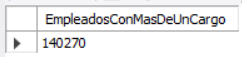
\includegraphics[width=0.5\textwidth]{imagenes/EmpleadosMasDeUnCargo.png}
\caption{Resultado -- Empleados con Más de un Cargo}
\end{figure}

\subsubsection{¿Qué departamentos presentan mayor movilidad interna?}
\textbf{Necesidad de Negocio:} Mapear el crecimiento profesional e identificar qué departamentos lideran el desarrollo interno.

\textbf{SQL QUERY:}
\begin{lstlisting}[language=SQL, caption={Consulta -- Tasa de Movilidad Interna por Departamento}]
SELECT
    d.dept_name AS Departamento,
    COUNT(*) AS TotalEmpleados,
    SUM(CASE WHEN p.emp_no IS NOT NULL THEN 1 ELSE 0 END) AS EmpleadosConMasDeUnCargo,
    ROUND(
        SUM(CASE WHEN p.emp_no IS NOT NULL THEN 1 ELSE 0 END) * 100.0 / COUNT(*),
        2
    ) AS TasaMovilidad
FROM employees.dept_emp de
JOIN employees.departments d
    ON de.dept_no = d.dept_no
LEFT JOIN (
    SELECT emp_no
    FROM employees.titles
    GROUP BY emp_no
    HAVING COUNT(DISTINCT title) > 1
) p ON de.emp_no = p.emp_no
WHERE de.from_date <= '2002-12-31'
  AND de.to_date > '2002-12-31'
GROUP BY d.dept_name
ORDER BY TasaMovilidad DESC;
\end{lstlisting}

\textbf{Hallazgos:}

Los resultados muestran que el departamento con la \textbf{mayor tasa de movilidad interna} es \textbf{Finance}, con un \textbf{57.14\%} de sus empleados habiendo ocupado más de un cargo. Le siguen \textbf{Human Resources} con \textbf{56.88\%}, \textbf{Sales} con \textbf{56.27\%} y \textbf{Marketing} con \textbf{56.16\%}. En contraste, el departamento con la tasa más baja es \textbf{Quality Management}, con \textbf{50.61\%}. En general, todos los departamentos presentan tasas superiores al \textbf{50\%}.

\textbf{Insights:}

Este comportamiento sugiere que la movilidad interna es una práctica extendida en toda la empresa y no un fenómeno aislado. Aunque \textbf{Finance}, \textbf{Human Resources} y \textbf{Sales} destacan como las áreas con mayor dinamismo, la diferencia respecto a otros departamentos no es muy amplia, lo que apunta a una cultura organizacional donde el desarrollo interno está relativamente distribuido. Sería valioso analizar si estos movimientos corresponden principalmente a promociones verticales, cambios laterales o ajustes operativos.

\begin{figure}[H]
\centering
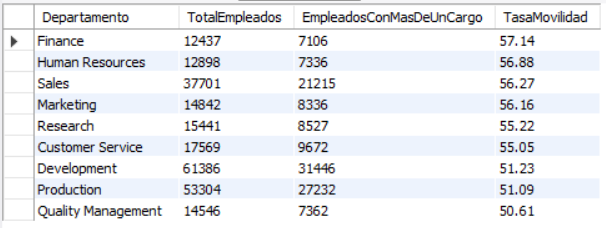
\includegraphics[width=0.8\textwidth]{imagenes/PromocionYTasas.png}
\caption{Resultado -- Tasa de Movilidad Interna por Departamento}
\end{figure}

\subsubsection{¿Cuánto tiempo suelen permanecer los empleados en su primer rol antes de ser promovidos?}
\textbf{Necesidad de Negocio:} Medir la velocidad del crecimiento profesional y la agilidad de las carreras internas.

\textbf{SQL QUERY:}
\begin{lstlisting}[language=SQL, caption={Consulta -- Tiempo Promedio en el Primer Rol}]
SELECT
    ROUND(AVG(DATEDIFF(t.to_date, t.from_date) / 365.25), 2) AS PromedioAniosPrimerRol
FROM employees.titles t
JOIN (
    SELECT emp_no, MIN(from_date) AS PrimerFromDate
    FROM employees.titles
    GROUP BY emp_no
) primer_rol
    ON t.emp_no = primer_rol.emp_no
   AND t.from_date = primer_rol.PrimerFromDate
WHERE t.to_date <> '9999-01-01'
  AND t.to_date <= '2002-12-31'
  AND t.emp_no IN (
      SELECT emp_no
      FROM employees.titles
      GROUP BY emp_no
      HAVING COUNT(DISTINCT title) > 1
  );
\end{lstlisting}

\textbf{Hallazgos:}

La consulta indica que los empleados que han cambiado de puesto permanecieron en su \textbf{primer rol un promedio de 6.79 años} antes de ser promovidos o moverse a un cargo distinto dentro de la organización.

\textbf{Insights:}

Este resultado sugiere que el crecimiento interno ocurre en un horizonte de mediano a largo plazo. Un promedio de \textbf{6.79 años} en el primer rol puede interpretarse como una trayectoria que valora la acumulación de experiencia antes de asumir nuevas responsabilidades. Para Recursos Humanos, este indicador puede servir como referencia para evaluar si los procesos de promoción son consistentes con la estrategia organizacional o si existen oportunidades para acelerar la evolución profesional en ciertas áreas.

\begin{figure}[H]
\centering
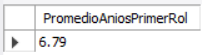
\includegraphics[width=0.35\textwidth]{imagenes/AniosPrimeraPromocion.png}
\caption{Resultado -- Tiempo Promedio en el Primer Rol}
\end{figure}


\subsection{Retención y Antigüedad}

\subsubsection{¿Cuál es la antigüedad promedio de los empleados en la empresa?}
\textbf{Necesidad de Negocio:} Evaluar la lealtad general y la estabilidad dentro de la organización.

\textbf{SQL QUERY:}
\begin{lstlisting}[language=SQL, caption={Consulta -- Antigüedad Promedio de Empleados}]
SELECT
    ROUND(AVG(DATEDIFF('2002-12-31', e.hire_date) / 365.25), 2) AS AntiguedadPromedioAnios
FROM employees.employees e
JOIN employees.dept_emp de ON e.emp_no = de.emp_no
WHERE de.from_date <= '2002-12-31'
  AND de.to_date > '2002-12-31';
\end{lstlisting}

\textbf{Hallazgos:}

La consulta muestra que la \textbf{antigüedad promedio} de los empleados activos al \textbf{31 de diciembre de 2002} es de \textbf{12.92 años} dentro de la empresa.

\textbf{Insights:}

Este resultado sugiere que la organización cuenta con una fuerza laboral relativamente estable y con una permanencia significativa en el tiempo. Una antigüedad promedio de \textbf{12.92 años} puede interpretarse como un indicador de lealtad organizacional, experiencia acumulada y continuidad operativa. Desde una perspectiva de negocio, este comportamiento puede generar beneficios en términos de retención de conocimiento y especialización; sin embargo, también vuelve relevante analizar si la empresa está equilibrando la permanencia del talento con la incorporación de nuevos perfiles.

\begin{figure}[H]
\centering
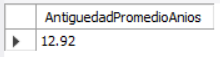
\includegraphics[width=0.35\textwidth]{imagenes/AntiguedadPromedio.png}
\caption{Resultado -- Antigüedad Promedio de Empleados}
\end{figure}

\subsubsection{¿Qué departamentos tienen la mayor y menor retención?}
\textbf{Necesidad de Negocio:} Detectar posibles problemas de liderazgo o cultura en áreas específicas.

\textbf{SQL QUERY:}
\begin{lstlisting}[language=SQL, caption={Consulta -- Antigüedad Promedio por Departamento}]
SELECT
    d.dept_name AS Departamento,
    COUNT(*) AS TotalEmpleados,
    ROUND(AVG(DATEDIFF('2002-12-31', e.hire_date) / 365.25), 2) AS AntiguedadPromedioAnios
FROM employees.employees e
JOIN employees.dept_emp de ON e.emp_no = de.emp_no
JOIN employees.departments d ON de.dept_no = d.dept_no
WHERE de.from_date <= '2002-12-31'
  AND de.to_date > '2002-12-31'
GROUP BY d.dept_name
ORDER BY AntiguedadPromedioAnios DESC;
\end{lstlisting}

\textbf{Hallazgos:}

Tomando la \textbf{antigüedad promedio} como una aproximación de la retención por departamento, los resultados muestran que \textbf{Finance} y \textbf{Production} presentan el valor más alto, con \textbf{12.93 años}. Por otro lado, \textbf{Marketing} y \textbf{Quality Management} registran el valor más bajo, con \textbf{12.90 años}. La diferencia entre el valor más alto y el más bajo es de únicamente \textbf{0.03 años}.

\textbf{Insights:}

Los resultados sugieren que la retención es \textbf{altamente uniforme} en toda la organización. Desde una perspectiva de negocio, esto indica que no existe evidencia clara de problemas severos de liderazgo o clima laboral concentrados en un área específica, al menos bajo esta métrica. Sería conveniente complementar el estudio con indicadores más directos de rotación o salida para profundizar en las causas de permanencia o abandono por área.

\begin{figure}[H]
\centering
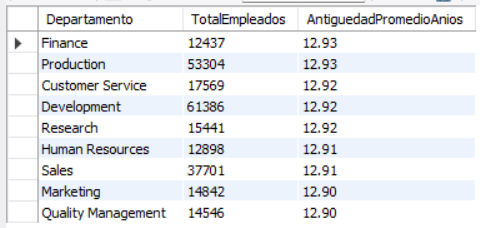
\includegraphics[width=0.7\textwidth]{imagenes/AntiguedadDepartamentos.png}
\caption{Resultado -- Antigüedad Promedio por Departamento}
\end{figure}


\subsection{Tendencias de Contratación}

\subsubsection{¿Cuántos empleados fueron contratados cada año y mes?}
\textbf{Necesidad de Negocio:} Rastrear el crecimiento de las contrataciones e identificar patrones estacionales.

\begin{lstlisting}[language=SQL, caption={Consulta -- Contrataciones por Año}]
SELECT
    YEAR(hire_date) AS AnioContratacion,
    COUNT(*) AS NumContrataciones
FROM employees.employees
GROUP BY YEAR(hire_date)
ORDER BY AnioContratacion;
\end{lstlisting}

\begin{lstlisting}[language=SQL, caption={Consulta -- Contrataciones por Mes}]
SELECT
    MONTH(hire_date) AS MesContratacion,
    COUNT(*) AS NumContrataciones
FROM employees.employees
GROUP BY MONTH(hire_date)
ORDER BY MesContratacion;
\end{lstlisting}

\textbf{Hallazgos:}

El mayor volumen de incorporación ocurrió en los primeros años del periodo: \textbf{1986} con \textbf{36150 contrataciones}, \textbf{1985} con \textbf{35316} y \textbf{1987} con \textbf{33501}. A partir de ese punto, las contrataciones presentan una tendencia descendente sostenida hasta llegar a \textbf{1514} en 1999 y únicamente \textbf{13} en 2000. Por mes, \textbf{marzo} es el más activo con \textbf{26917 contrataciones} y \textbf{enero} el más bajo con \textbf{23859}.

\textbf{Insights:}

Los resultados sugieren que el crecimiento de la plantilla fue mucho más intenso en las etapas iniciales, seguido por una fase de estabilización. En cuanto al comportamiento mensual, no se identifica una estacionalidad extremadamente marcada; las contrataciones se distribuyen de manera relativamente uniforme a lo largo del año.

\begin{figure}[H]
\centering
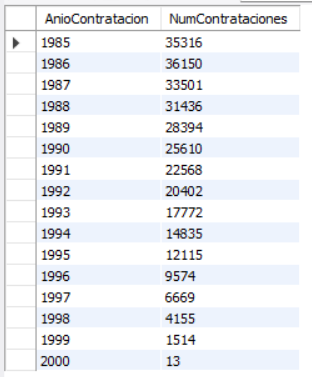
\includegraphics[width=0.7\textwidth]{imagenes/ContratacionesPorAnio.png}
\caption{Resultado -- Contrataciones por Año}
\end{figure}

\begin{figure}[H]
\centering
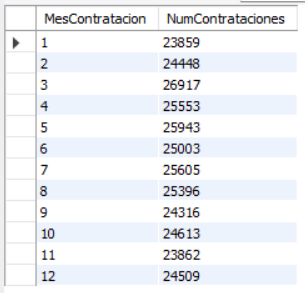
\includegraphics[width=0.7\textwidth]{imagenes/ContratacionesPorMes.png}
\caption{Resultado -- Contrataciones por Mes}
\end{figure}

\subsubsection{¿Cuáles son los días de la semana más comunes para las contrataciones?}
\textbf{Necesidad de Negocio:} Identificar patrones operativos en los procesos de reclutamiento e incorporación.

\textbf{SQL QUERY:}
\begin{lstlisting}[language=SQL, caption={Consulta -- Contrataciones por Día de la Semana}]
SELECT
    CASE DAYOFWEEK(hire_date)
        WHEN 1 THEN 'Domingo'
        WHEN 2 THEN 'Lunes'
        WHEN 3 THEN 'Martes'
        WHEN 4 THEN 'Miercoles'
        WHEN 5 THEN 'Jueves'
        WHEN 6 THEN 'Viernes'
        WHEN 7 THEN 'Sabado'
    END AS DiaSemana,
    COUNT(*) AS NumContrataciones
FROM employees.employees
GROUP BY 
    DAYOFWEEK(hire_date),
    CASE DAYOFWEEK(hire_date)
        WHEN 1 THEN 'Domingo'
        WHEN 2 THEN 'Lunes'
        WHEN 3 THEN 'Martes'
        WHEN 4 THEN 'Miercoles'
        WHEN 5 THEN 'Jueves'
        WHEN 6 THEN 'Viernes'
        WHEN 7 THEN 'Sabado'
    END
ORDER BY DAYOFWEEK(hire_date);
\end{lstlisting}

\textbf{Hallazgos:}

El día con mayor número de contrataciones es \textbf{sábado} con \textbf{42918} registros, seguido por \textbf{lunes} con \textbf{42916}. El día con menor número es \textbf{domingo} con \textbf{42527}. Las diferencias entre días son mínimas, todas cercanas a las \textbf{42 mil} incorporaciones.

\textbf{Insights:}

No existe un patrón operativo fuertemente marcado en torno a un solo día de la semana para las contrataciones. El proceso de incorporación parece estar distribuido de forma bastante uniforme a lo largo de la semana, lo que indica que los procesos de reclutamiento operan de manera relativamente constante.

\begin{figure}[H]
\centering
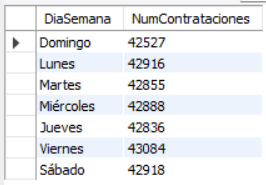
\includegraphics[width=0.7\textwidth]{imagenes/ContratacionesPorDia.png}
\caption{Resultado -- Contrataciones por Día de la Semana}
\end{figure}

\newpage

%%%%%%%%%%%%%%%%%%%%%%%%%%%%%%%%%%%%%%%%%%%%%
\section{Parte 2: Perspectivas Salariales}
%%%%%%%%%%%%%%%%%%%%%%%%%%%%%%%%%%%%%%%%%%%%%

\subsection{Estadísticas Salariales Generales}

\subsubsection{¿Cuál es el salario promedio y cómo ha evolucionado?}
\textbf{Necesidad de Negocio:} Evaluar la competitividad y rastrear el crecimiento salarial a lo largo del tiempo.

\begin{lstlisting}[language=SQL, caption={Consulta -- Salario Promedio Vigente}]
SELECT
    ROUND(AVG(salary), 2) AS SalarioPromedio
FROM employees.salaries
WHERE from_date <= '2002-12-31'
  AND to_date > '2002-12-31';
\end{lstlisting}

\begin{lstlisting}[language=SQL, caption={Consulta -- Evolución Anual del Salario Promedio}]
SELECT
    YEAR(from_date) AS Anio,
    ROUND(AVG(salary), 2) AS SalarioPromedio
FROM employees.salaries
GROUP BY YEAR(from_date)
ORDER BY Anio;
\end{lstlisting}

\textbf{Hallazgos:}

El \textbf{salario promedio vigente al 31 de diciembre de 2002} es de \textbf{71964.80}. En la evolución histórica, el promedio pasó de \textbf{53419.78} en 1985 hasta \textbf{72622.59} en 2001, reflejando un incremento progresivo en la compensación promedio durante todo el periodo analizado.

\textbf{Insights:}

La empresa ha mantenido una trayectoria ascendente en su política de compensación, lo cual puede interpretarse como una señal de ajuste salarial continuo y de fortalecimiento de su competitividad interna. Este comportamiento puede asociarse con estrategias de retención, reconocimiento de experiencia acumulada o adaptación a condiciones del mercado laboral.

\begin{figure}[H]
\centering
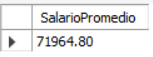
\includegraphics[width=0.25\textwidth]{imagenes/SalarioPromedio.png}
\caption{Resultado -- Salario Promedio Vigente}
\end{figure}

\begin{figure}[H]
\centering
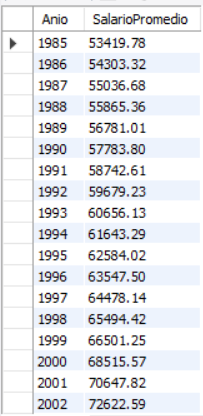
\includegraphics[width=0.35\textwidth]{imagenes/EvolucionSalarioPromedio.png}
\caption{Resultado -- Evolución Anual del Salario Promedio}
\end{figure}

\subsubsection{¿Cuál es el salario más alto y más bajo de la empresa?}
\textbf{Necesidad de Negocio:} Conocer el rango salarial completo para benchmarking interno y definición de bandas salariales.

\textbf{SQL QUERY:}
\begin{lstlisting}[language=SQL, caption={Consulta -- Salario Máximo y Mínimo}]
SELECT 
    MAX(salary) AS SalarioMaximo,
    MIN(salary) AS SalarioMinimo
FROM salaries
WHERE to_date = '9999-01-01';
\end{lstlisting}

\textbf{Hallazgos:}

El salario máximo registrado es de \textbf{\$158,220} y el salario mínimo es de \textbf{\$39,012}. Existe una diferencia de \textbf{\$119,208} entre ambos extremos.

\textbf{Insights:}

El amplio rango salarial refleja una estructura con distintos niveles jerárquicos y especialización. Este dato es útil para benchmarking y para definir bandas salariales internas que garanticen equidad y competitividad en cada nivel.

\begin{figure}[H]
\centering
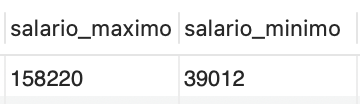
\includegraphics[width=0.4\textwidth]{imagenes/SalarioMaximoMinimo.png}
\caption{Resultado -- Salario Máximo y Mínimo}
\end{figure}

\subsubsection{¿Cuál es la desviación estándar de los salarios?}
\textbf{Necesidad de Negocio:} Medir la dispersión salarial para entender qué tan homogénea es la distribución de sueldos.

\textbf{SQL QUERY:}
\begin{lstlisting}[language=SQL, caption={Consulta -- Desviación Estándar de Salarios}]
SELECT 
    ROUND(STDDEV(salary), 2) AS DesviacionEstandar
FROM salaries
WHERE to_date = '9999-01-01';
\end{lstlisting}

\textbf{Hallazgos:}

La desviación estándar de los salarios es de \textbf{\$17,332.02}.

\textbf{Insights:}

Comparada con el salario promedio (\$71,964.80), el coeficiente de variación es de aproximadamente \textbf{24\%}, lo que indica una dispersión moderada. Los salarios no están demasiado concentrados alrededor del promedio, lo cual es consistente con una empresa que tiene diversos niveles jerárquicos.

\begin{figure}[H]
\centering
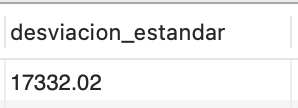
\includegraphics[width=0.4\textwidth]{imagenes/DesviacionEstandarSalarios.png}
\caption{Resultado -- Desviación Estándar de Salarios}
\end{figure}

\subsubsection{¿Cuál es el salario más frecuente en la empresa?}
\textbf{Necesidad de Negocio:} Identificar el salario más común para entender la concentración salarial en la plantilla.

\textbf{SQL QUERY:}
\begin{lstlisting}[language=SQL, caption={Consulta -- Salario Más Frecuente}]
SELECT 
    salary,
    COUNT(*) AS Frecuencia
FROM salaries
WHERE to_date = '9999-01-01'
GROUP BY salary
ORDER BY Frecuencia DESC
LIMIT 1;
\end{lstlisting}

\textbf{Hallazgos:}

El salario más frecuente es \textbf{\$71,669}, con \textbf{9 empleados} percibiéndolo.

\textbf{Insights:}

Este valor es muy cercano al promedio general (\$71,964.80), lo que sugiere que existe una banda salarial central donde se concentra buena parte de los empleados de nivel medio.

\begin{figure}[H]
\centering
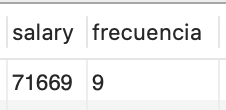
\includegraphics[width=0.4\textwidth]{imagenes/SalarioFrecuente.png}
\caption{Resultado -- Salario Más Frecuente}
\end{figure}


\subsection{Segmentos Salariales}

\subsubsection{¿Cuántos empleados ganan más de \$100,000?}
\textbf{Necesidad de Negocio:} Identificar el segmento de altos ingresos para diseñar planes de retención diferenciados.

\textbf{SQL QUERY:}
\begin{lstlisting}[language=SQL, caption={Consulta -- Empleados con Salario Mayor a \$100{,}000}]
SELECT 
    COUNT(*) AS EmpleadosMas100k
FROM salaries
WHERE to_date = '9999-01-01'
  AND salary > 100000;
\end{lstlisting}

\textbf{Hallazgos:}

\textbf{5,927 empleados} ganan más de \$100,000 anuales.

\textbf{Insights:}

Este grupo representa el segmento de altos ingresos de la empresa y es clave para estrategias de retención, ya que suelen ser perfiles con alta demanda en el mercado.

\begin{figure}[H]
\centering
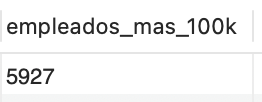
\includegraphics[width=0.4\textwidth]{imagenes/EmpleadosMas100k.png}
\caption{Resultado -- Empleados con Salario Mayor a \$100,000}
\end{figure}

\subsubsection{¿Cuáles son los 5 salarios más altos de la empresa?}
\textbf{Necesidad de Negocio:} Identificar a los top earners para diseñar planes de retención y sucesión personalizados.

\textbf{SQL QUERY:}
\begin{lstlisting}[language=SQL, caption={Consulta -- Top 5 Salarios más Altos}]
SELECT 
    emp_no,
    salary
FROM salaries
WHERE to_date = '9999-01-01'
ORDER BY salary DESC
LIMIT 5;
\end{lstlisting}

\textbf{Hallazgos:}

Los cinco salarios más altos de la empresa oscilan entre \textbf{\$150,345} y \textbf{\$158,220}.

\textbf{Insights:}

Los top earners están concentrados en un rango de \$150K--\$158K. Identificar a estos empleados permite a RH diseñar planes de retención personalizados y planes de sucesión.

\begin{figure}[H]
\centering
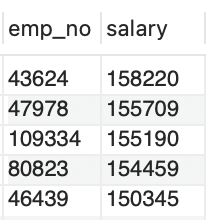
\includegraphics[width=0.5\textwidth]{imagenes/Top5Salarios.png}
\caption{Resultado -- Top 5 Salarios más Altos}
\end{figure}

\subsubsection{¿Cuántos empleados ganan menos de \$50,000?}
\textbf{Necesidad de Negocio:} Identificar la base salarial más vulnerable para evaluar riesgo de rotación en niveles de entrada.

\textbf{SQL QUERY:}
\begin{lstlisting}[language=SQL, caption={Consulta -- Empleados con Salario Menor a \$50{,}000}]
SELECT 
    COUNT(*) AS EmpleadosMenos50k
FROM salaries
WHERE to_date = '9999-01-01'
  AND salary < 50000;
\end{lstlisting}

\textbf{Hallazgos:}

\textbf{6,960 empleados} ganan menos de \$50,000 anuales.

\textbf{Insights:}

Este segmento representa la base salarial más vulnerable. RH debería revisar si estos salarios son competitivos respecto al mercado para reducir el riesgo de rotación en posiciones de entrada.

\begin{figure}[H]
\centering
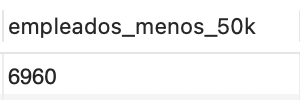
\includegraphics[width=0.4\textwidth]{imagenes/EmpleadosMenos50k.png}
\caption{Resultado -- Empleados con Salario Menor a \$50,000}
\end{figure}


\subsection{Análisis de Nómina}

\subsubsection{¿Cuál es el gasto total de nómina de la empresa?}
\textbf{Necesidad de Negocio:} Conocer el costo base de nómina para la planeación financiera y presupuestaria.

\textbf{SQL QUERY:}
\begin{lstlisting}[language=SQL, caption={Consulta -- Gasto Total de Nómina}]
SELECT 
    SUM(salary) AS NominaTotal
FROM salaries
WHERE to_date = '9999-01-01';
\end{lstlisting}

\textbf{Hallazgos:}

La nómina total asciende a \textbf{\$5,874,846,442 USD anuales} (~\$5.87 mil millones).

\textbf{Insights:}

Este es el costo base para la planeación financiera. Sirve como referencia para proyectar aumentos anuales, bonos y presupuesto de nuevas contrataciones.

\begin{figure}[H]
\centering
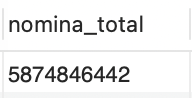
\includegraphics[width=0.4\textwidth]{imagenes/NominaTotal.png}
\caption{Resultado -- Gasto Total de Nómina}
\end{figure}

\subsubsection{¿Cuál es la nómina total de empleados que ganan más de \$90,000?}
\textbf{Necesidad de Negocio:} Evaluar el impacto financiero de los perfiles senior en el gasto total de nómina.

\textbf{SQL QUERY:}
\begin{lstlisting}[language=SQL, caption={Consulta -- Nómina de Empleados con Salario Mayor a \$90{,}000}]
SELECT 
    SUM(salary) AS NominaAltosIngresos
FROM salaries
WHERE to_date = '9999-01-01'
  AND salary > 90000;
\end{lstlisting}

\textbf{Hallazgos:}

La nómina de empleados con salario superior a \$90,000 asciende a \textbf{\$1,294,918,949 USD anuales} (~\$1.29 mil millones).

\textbf{Insights:}

Los altos ingresos representan aproximadamente el \textbf{22\%} del gasto total de nómina, a pesar de ser una porción menor de la plantilla. Este dato es crítico para evaluar el impacto financiero de políticas de compensación en niveles senior.

\begin{figure}[H]
\centering
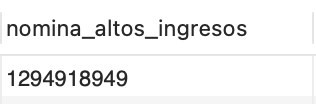
\includegraphics[width=0.4\textwidth]{imagenes/NominaAltosIngresos.png}
\caption{Resultado -- Nómina de Empleados con Salario Mayor a \$90,000}
\end{figure}

\subsubsection{¿Cuánto gasta la empresa anualmente en salarios mayores a \$80,000?}
\textbf{Necesidad de Negocio:} Controlar el crecimiento del gasto en niveles salariales altos.

\textbf{SQL QUERY:}
\begin{lstlisting}[language=SQL, caption={Consulta -- Gasto Anual en Salarios Mayores a \$80{,}000}]
SELECT 
    YEAR(from_date) AS anio,
    SUM(salary) AS gasto_total_salarios_altos
FROM salaries
WHERE salary > 80000
GROUP BY YEAR(from_date)
ORDER BY anio DESC;
\end{lstlisting}

\textbf{Hallazgos:}

El gasto anual en salarios superiores a \$80,000 ha mostrado un crecimiento constante a lo largo de los años, iniciando en \textbf{\$34,043,565 USD} en 1985 y alcanzando un pico histórico de \textbf{\$2,107,422,272 USD} (~\$2.11 mil millones) en el año 2001. Para el año 2002, el registro cierra en \textbf{\$1,351,008,401 USD} debido al corte de registros en el historial de la base de datos.

\textbf{Insights:}

La evolución de los datos refleja una expansión masiva y acelerada en la nómina de alta compensación, multiplicándose el gasto por más de 60 veces entre 1985 y 2001. Este incremento exponencial en los años noventa señala que los salarios altos pasaron a concentrar una parte crítica del costo operativo, lo que obliga a las áreas de RH y Finanzas a monitorear la tasa de retención de perfiles senior y planear estrategias de compensación sostenibles a largo plazo.

\begin{figure}[H]
\centering
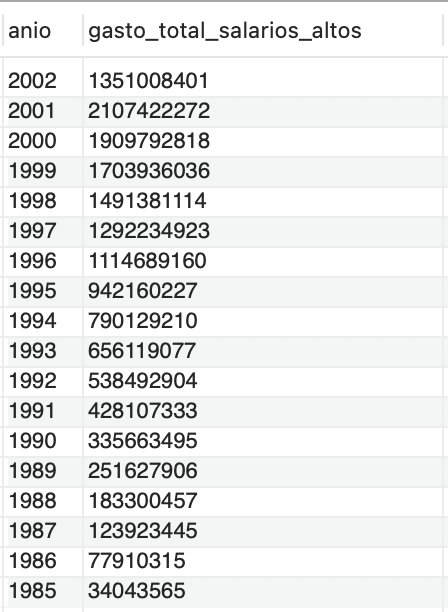
\includegraphics[width=0.4\textwidth]{imagenes/GastoSalarios80k.png}
\caption{Resultado -- Gasto Anual en Salarios Mayores a \$80,000}
\end{figure}


\subsection{Equidad Salarial}

\subsubsection{¿Existe una brecha salarial por género?}
\textbf{Necesidad de Negocio:} Verificar que la empresa garantiza equidad salarial entre géneros.

\textbf{SQL QUERY:}
\begin{lstlisting}[language=SQL, caption={Consulta -- Brecha Salarial por Género}]
SELECT 
    e.gender,
    ROUND(AVG(s.salary), 2) AS SalarioPromedio,
    COUNT(*) AS TotalEmpleados
FROM salaries s
JOIN employees e ON s.emp_no = e.emp_no
WHERE s.to_date = '9999-01-01'
GROUP BY e.gender;
\end{lstlisting}

\textbf{Hallazgos:}

El salario promedio masculino es de \textbf{\$71,990.47} (48,927 empleados) y el femenino de \textbf{\$71,926.40} (32,708 empleados). La diferencia es de apenas \textbf{\$64.07 (0.09\%)}.

\textbf{Insights:}

La brecha salarial es prácticamente inexistente, lo cual es un hallazgo muy positivo. Sin embargo, se observa un desbalance en la representación: los hombres representan ~60\% de la plantilla vs. 40\% mujeres. RH podría enfocarse en iniciativas de diversidad e inclusión para balancear la fuerza laboral.

\begin{figure}[H]
\centering
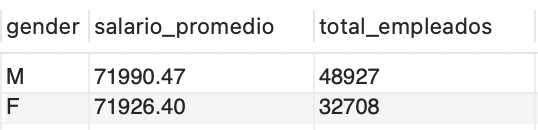
\includegraphics[width=0.5\textwidth]{imagenes/BrechaSalarialGenero.png}
\caption{Resultado -- Brecha Salarial por Género}
\end{figure}


\subsection{Salarios por Departamento y Puesto}

\subsubsection{¿Qué departamentos o puestos tienen los promedios salariales más altos?}
\textbf{Necesidad de Negocio:} Entender la distribución de los costos laborales en las diferentes áreas.

\begin{lstlisting}[language=SQL, caption={Consulta -- Salario Promedio por Departamento}]
SELECT
    d.dept_name AS Departamento,
    COUNT(*) AS TotalEmpleados,
    ROUND(AVG(s.salary), 2) AS SalarioPromedio
FROM employees.salaries s
JOIN employees.dept_emp de ON s.emp_no = de.emp_no
JOIN employees.departments d ON de.dept_no = d.dept_no
WHERE s.from_date <= '2002-12-31'
  AND s.to_date > '2002-12-31'
  AND de.from_date <= '2002-12-31'
  AND de.to_date > '2002-12-31'
GROUP BY d.dept_name
ORDER BY SalarioPromedio DESC;
\end{lstlisting}

\begin{lstlisting}[language=SQL, caption={Consulta -- Salario Promedio por Puesto}]
SELECT
    t.title AS Puesto,
    COUNT(*) AS TotalEmpleados,
    ROUND(AVG(s.salary), 2) AS SalarioPromedio
FROM employees.salaries s
JOIN employees.titles t ON s.emp_no = t.emp_no
WHERE s.from_date <= '2002-12-31'
  AND s.to_date > '2002-12-31'
  AND t.from_date <= '2002-12-31'
  AND t.to_date > '2002-12-31'
GROUP BY t.title
ORDER BY SalarioPromedio DESC;
\end{lstlisting}

\textbf{Hallazgos:}

En el análisis por departamento, \textbf{Sales} presenta el \textbf{salario promedio más alto}, con \textbf{89005.79}, seguido por \textbf{Marketing} con \textbf{79879.18} y \textbf{Finance} con \textbf{78075.46}. En contraste, los departamentos con los promedios salariales más bajos son \textbf{Human Resources}, con \textbf{63643.26}, y \textbf{Quality Management}, con \textbf{65516.97}.

Por otra parte, en el análisis por puesto, el promedio salarial más alto corresponde a \textbf{Senior Staff}, con \textbf{80584.05}, seguido por \textbf{Manager}, con \textbf{77723.67}, y \textbf{Senior Engineer}, con \textbf{70845.33}. En los niveles más bajos aparecen \textbf{Engineer}, con \textbf{59590.07}, y \textbf{Assistant Engineer}, con \textbf{57504.68}. Cabe señalar que el puesto de \textbf{Manager} cuenta con únicamente \textbf{9 empleados}, por lo que su promedio debe interpretarse con cierta cautela.

\textbf{Insights:}

Los costos salariales no se distribuyen de manera homogénea. A nivel departamental, áreas como \textbf{Sales}, \textbf{Marketing} y \textbf{Finance} concentran los promedios más elevados, asociados con funciones de mayor impacto comercial o estratégico. A nivel de puesto, los salarios más altos se concentran en roles senior, lo que sugiere que la estructura de compensación está alineada con la jerarquía organizacional.

\begin{figure}[H]
\centering
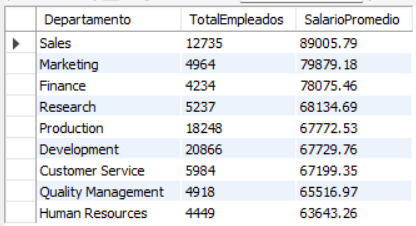
\includegraphics[width=0.6\textwidth]{imagenes/SalariosPorDepartamento.png}
\caption{Resultado -- Salario Promedio por Departamento}
\end{figure}

\begin{figure}[H]
\centering
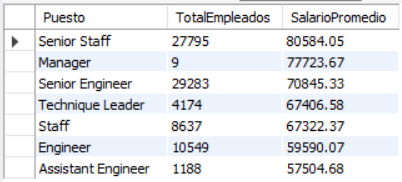
\includegraphics[width=0.6\textwidth]{imagenes/SalariosPorPuesto.png}
\caption{Resultado -- Salario Promedio por Puesto}
\end{figure}

\newpage

%%%%%%%%%%%%%%%%%%%%%%%%%%%%%%%%%%%%%%%%%%%%%
\section{Parte 3: Desempeño Departamental}
%%%%%%%%%%%%%%%%%%%%%%%%%%%%%%%%%%%%%%%%%%%%%

\subsection{Distribución de la Fuerza Laboral por Departamento}

\subsubsection{¿Cómo se distribuye la fuerza laboral entre departamentos y cuál es el más grande?}
\textbf{Necesidad de Negocio:} Entender cómo están distribuidos los recursos humanos para apoyar decisiones de presupuesto y contratación por área.

\textbf{SQL QUERY:}
\begin{lstlisting}[language=SQL, caption={Consulta -- Distribución de Empleados por Departamento}]
SELECT 
    d.dept_name AS Departamento,
    COUNT(de.emp_no) AS TotalEmpleados
FROM dept_emp de
JOIN departments d ON de.dept_no = d.dept_no
WHERE de.from_date <= '2002-12-31'
  AND de.to_date > '2002-12-31'
GROUP BY d.dept_name
ORDER BY TotalEmpleados DESC;
\end{lstlisting}

\textbf{Hallazgos:}

Los resultados muestran que \textbf{Development} es el departamento más grande con \textbf{61,386 empleados}, seguido por \textbf{Production} con \textbf{53,304}. Entre ambos concentran más del \textbf{50\%} de la fuerza laboral activa. En el extremo opuesto, \textbf{Finance} es el departamento más pequeño con \textbf{12,437 empleados}, seguido por \textbf{Human Resources} con \textbf{12,898}.

\textbf{Insights:}

La distribución refleja una empresa claramente orientada hacia tecnología y producción. El hecho de que dos departamentos concentren más de la mitad de la plantilla tiene implicaciones importantes para la asignación de presupuesto, la planificación de contrataciones y la priorización de programas de RH. Los departamentos más pequeños, como Finance y Human Resources, aunque críticos para la operación, representan una inversión de headcount comparativamente menor.

\begin{figure}[H]
\centering
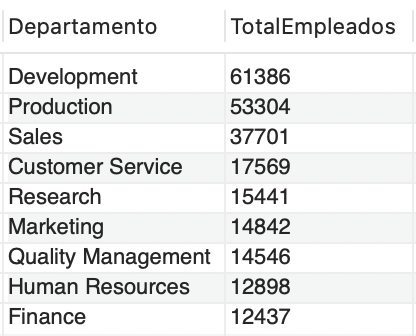
\includegraphics[width=0.7\textwidth]{imagenes/pregunta_3_1.png}
\caption{Resultado -- Distribución de Empleados por Departamento}
\end{figure}


\subsection{Estabilidad del Liderazgo Departamental}

\subsubsection{¿Qué departamentos han tenido más cambios de gerente?}
\textbf{Necesidad de Negocio:} Detectar inestabilidad en el liderazgo de áreas específicas que pueda impactar la cultura y retención.

\textbf{SQL QUERY:}
\begin{lstlisting}[language=SQL, caption={Consulta -- Cambios de Gerente por Departamento}]
SELECT 
    d.dept_name AS Departamento,
    COUNT(*) AS CambiosDeGerente
FROM dept_manager dm
JOIN departments d ON dm.dept_no = d.dept_no
GROUP BY d.dept_name
ORDER BY CambiosDeGerente DESC;
\end{lstlisting}

\textbf{Hallazgos:}

Los departamentos con mayor número de cambios de gerente son \textbf{Customer Service}, \textbf{Quality Management} y \textbf{Production}, cada uno con \textbf{4 cambios}. El resto de los departamentos (\textbf{Development}, \textbf{Marketing}, \textbf{Research}, \textbf{Human Resources}, \textbf{Finance} y \textbf{Sales}) registran únicamente \textbf{2 cambios} de gerente a lo largo de su historia.

\textbf{Insights:}

La mayor rotación de liderazgo en \textbf{Customer Service}, \textbf{Quality Management} y \textbf{Production} podría ser señal de mayor exigencia operativa, mayor presión por resultados o menor estabilidad en estas áreas. Para Recursos Humanos, este hallazgo es relevante porque la continuidad del liderazgo impacta directamente en la cultura departamental, la retención de talento y la ejecución de planes de largo plazo. Vale la pena analizar si estos cambios fueron motivados por rotación voluntaria, promociones o bajo desempeño, ya que cada causa requiere una respuesta diferente.

\begin{figure}[H]
\centering
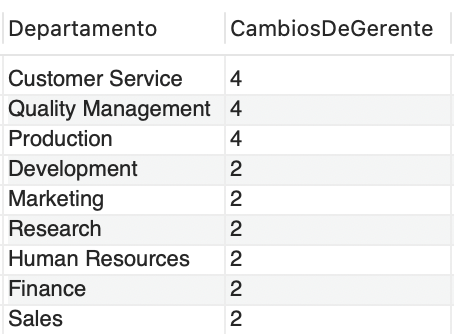
\includegraphics[width=0.6\textwidth]{imagenes/pregunt_3_2.png}
\caption{Resultado -- Cambios de Gerente por Departamento}
\end{figure}

\subsubsection{¿Cuál es la antigüedad de los gerentes actuales en cada departamento?}
\textbf{Necesidad de Negocio:} Identificar qué departamentos cuentan con liderazgo experimentado y cuáles con liderazgo más reciente.

\textbf{SQL QUERY:}
\begin{lstlisting}[language=SQL, caption={Consulta -- Antigüedad de Gerentes Actuales}]
SELECT 
    d.dept_name AS Departamento,
    CONCAT(e.first_name, ' ', e.last_name) AS NombreGerente,
    dm.from_date AS InicioComoGerente,
    ROUND(DATEDIFF('2002-12-31', dm.from_date) / 365.25, 2) AS AnosComoGerente
FROM dept_manager dm
JOIN departments d ON dm.dept_no = d.dept_no
JOIN employees e ON dm.emp_no = e.emp_no
WHERE dm.to_date > '2002-12-31'
ORDER BY AnosComoGerente DESC;
\end{lstlisting}

\textbf{Hallazgos:}

El gerente con mayor antigüedad en su puesto es \textbf{Isamu Legleitner} de \textbf{Finance}, con \textbf{13.04 años} en el cargo desde 1989. Le siguen \textbf{Hauke Zhang} de \textbf{Sales} con \textbf{11.82 años} y \textbf{Hilary Kambil} de \textbf{Research} con \textbf{11.73 años}. En el otro extremo, los gerentes más recientes son \textbf{Oscar Ghazalie} de \textbf{Production} con solo \textbf{6.34 años} y \textbf{Yuchang Weedman} de \textbf{Customer Service} con \textbf{6.99 años}.

\textbf{Insights:}

Este resultado es consistente con el análisis de cambios de gerente: los departamentos con más rotación de liderazgo (\textbf{Production} y \textbf{Customer Service}) son precisamente los que hoy tienen los gerentes más nuevos. Esto implica que estas áreas llevan relativamente poco tiempo bajo su liderazgo actual, lo que puede representar tanto un riesgo (menor experiencia acumulada en el rol) como una oportunidad (liderazgo fresco con nuevas perspectivas). En contraste, departamentos como \textbf{Finance} y \textbf{Sales} cuentan con líderes consolidados que aportan continuidad estratégica.

\begin{figure}[H]
\centering
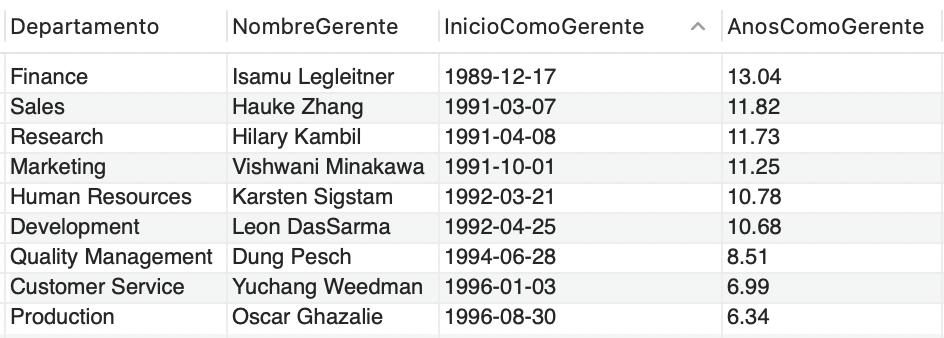
\includegraphics[width=\textwidth]{imagenes/preg_3_3.png}
\caption{Resultado -- Antigüedad de Gerentes Actuales}
\end{figure}


\subsection{Tendencias de Contratación Reciente por Departamento}

\subsubsection{¿Qué departamentos tuvieron más contrataciones en los últimos 5 años (1998--2002)?}
\textbf{Necesidad de Negocio:} Identificar dónde está ocurriendo el crecimiento más reciente para orientar el presupuesto de reclutamiento.

\textbf{SQL QUERY:}
\begin{lstlisting}[language=SQL, caption={Consulta -- Contrataciones por Departamento (1998--2002)}]
SELECT 
    d.dept_name AS Departamento,
    COUNT(*) AS ContratacionesUltimos5Anos
FROM employees e
JOIN dept_emp de ON e.emp_no = de.emp_no
JOIN departments d ON de.dept_no = d.dept_no
WHERE e.hire_date BETWEEN '1998-01-01' AND '2002-12-31'
GROUP BY d.dept_name
ORDER BY ContratacionesUltimos5Anos DESC;
\end{lstlisting}

\textbf{Hallazgos:}

En el período 1998--2002, \textbf{Development} lideró las contrataciones con \textbf{1,588 nuevos empleados}, seguido por \textbf{Production} con \textbf{1,363} y \textbf{Sales} con \textbf{973}. Los departamentos con menor actividad de contratación reciente fueron \textbf{Finance} con \textbf{331} y \textbf{Human Resources} con \textbf{340}.

\textbf{Insights:}

La tendencia de contratación reciente reproduce la distribución general de la empresa: \textbf{Development} y \textbf{Production} siguen siendo los motores de crecimiento en headcount. Esto es consistente con su posición como los departamentos más grandes. Para la dirección, este patrón puede interpretarse como una apuesta sostenida por fortalecer las áreas técnicas y de producción. \textbf{Finance} y \textbf{Human Resources}, pese a ser críticos para la operación, muestran el menor crecimiento en contrataciones recientes, lo que podría revisarse en función de las necesidades estratégicas de la empresa.

\begin{figure}[H]
\centering
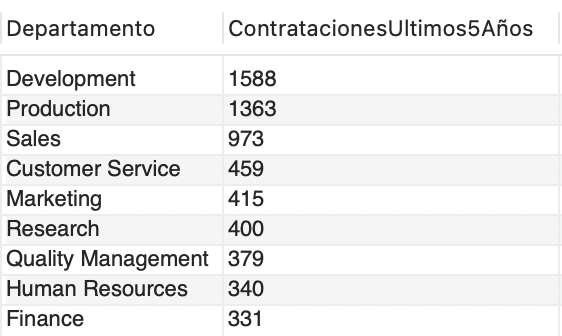
\includegraphics[width=0.7\textwidth]{imagenes/preg_3_4.png}
\caption{Resultado -- Contrataciones por Departamento (1998--2002)}
\end{figure}


\subsection{Retención por Departamento}

\subsubsection{¿Qué departamentos tienen la antigüedad promedio más baja?}
\textbf{Necesidad de Negocio:} Identificar áreas que podrían tener menor retención para diseñar intervenciones focalizadas.

\textbf{SQL QUERY:}
\begin{lstlisting}[language=SQL, caption={Consulta -- Antigüedad Promedio más Baja por Departamento}]
SELECT 
    d.dept_name AS Departamento,
    COUNT(*) AS TotalEmpleados,
    ROUND(AVG(DATEDIFF('2002-12-31', e.hire_date) / 365.25), 2) AS AntiguedadPromedioAnios
FROM employees e
JOIN dept_emp de ON e.emp_no = de.emp_no
JOIN departments d ON de.dept_no = d.dept_no
WHERE de.from_date <= '2002-12-31'
  AND de.to_date > '2002-12-31'
GROUP BY d.dept_name
ORDER BY AntiguedadPromedioAnios ASC;
\end{lstlisting}

\textbf{Hallazgos:}

Los departamentos con la antigüedad promedio más baja son \textbf{Marketing} y \textbf{Quality Management}, ambos con \textbf{12.90 años}, seguidos por \textbf{Sales} y \textbf{Human Resources} con \textbf{12.91 años}. En el extremo superior se encuentran \textbf{Finance} y \textbf{Production} con \textbf{12.93 años}. La diferencia total entre el valor más alto y el más bajo es de apenas \textbf{0.03 años}.

\textbf{Insights:}

La variación en antigüedad promedio entre departamentos es prácticamente inexistente, lo que confirma que la retención es uniforme en toda la organización al cierre de 2002. Ningún departamento muestra señales claras de problemas de retención basándose en esta métrica. Sin embargo, complementar este análisis con datos de bajas y rotación permitiría una visión más precisa.

\begin{figure}[H]
\centering
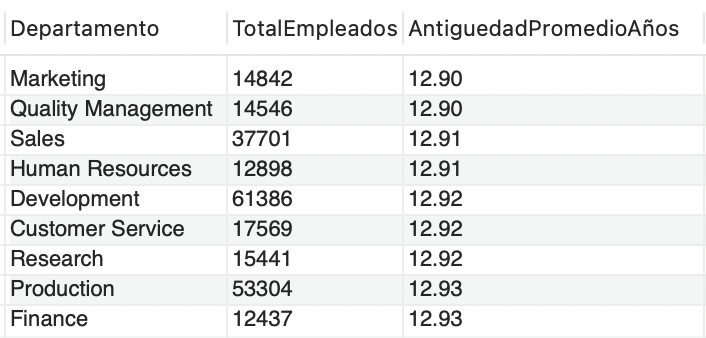
\includegraphics[width=0.7\textwidth]{imagenes/preg_3_5.png}
\caption{Resultado -- Antigüedad Promedio más Baja por Departamento}
\end{figure}


\newpage

%%%%%%%%%%%%%%%%%%%%%%%%%%%%%%%%%%%%%%%%%%%%%
\section{Conclusión y Recomendaciones}
%%%%%%%%%%%%%%%%%%%%%%%%%%%%%%%%%%%%%%%%%%%%%

Este análisis permitió comprender de manera integral la composición, estabilidad, movilidad, contratación, compensación y desempeño departamental de la fuerza laboral de la empresa. En conjunto, los resultados muestran una organización de gran escala, con una plantilla madura, estable y con una dinámica importante de crecimiento interno. Asimismo, se identificaron áreas de oportunidad relevantes para Recursos Humanos en materia de diversidad, desarrollo profesional, monitoreo de retención y revisión estratégica de la estructura salarial y el liderazgo departamental.

\subsubsection*{Hallazgos Clave}
\begin{itemize}
    \item \textbf{Tendencias de la fuerza laboral:} La empresa cuenta con \textbf{300024 empleados registrados}, una \textbf{edad promedio de 43.92 años} y una composición de género donde predominan los hombres (\textbf{59.99\%} frente a \textbf{40.01\%} de mujeres). Esto refleja una fuerza laboral amplia, madura y con oportunidades de mejora en equilibrio de género.

    \item \textbf{Movilidad y crecimiento:} Se identificó que \textbf{140270 empleados} han ocupado más de un cargo, lo que evidencia una práctica importante de movilidad interna. Los empleados que cambian de puesto permanecen en su primer rol un promedio de \textbf{6.79 años}, lo que sugiere trayectorias de crecimiento de mediano a largo plazo.

    \item \textbf{Retención y estabilidad:} La \textbf{antigüedad promedio} de los empleados activos es de \textbf{12.92 años}, lo que indica una organización con alta estabilidad laboral. A nivel departamental, la retención es muy uniforme, con diferencias de apenas \textbf{0.03 años} entre el departamento más y menos longevo.

    \item \textbf{Patrones de contratación:} Las contrataciones fueron mucho más altas en los primeros años del periodo y después mostraron una tendencia descendente sostenida. No se observan patrones estacionales fuertes por mes ni por día de la semana.

    \item \textbf{Compensación:} El salario promedio es de \textbf{\$71,964.80}, con una brecha salarial por género mínima (\textbf{0.09\%}). \textbf{Sales} lidera en salario promedio departamental (\$89,005.79) mientras que \textbf{Human Resources} presenta el más bajo (\$63,643.26).

    \item \textbf{Desempeño departamental:} \textbf{Development} y \textbf{Production} concentran más del 50\% de la fuerza laboral y lideran las contrataciones recientes, confirmando su rol central en la estrategia de la empresa. \textbf{Customer Service}, \textbf{Quality Management} y \textbf{Production} muestran mayor rotación de liderazgo con \textbf{4 cambios de gerente}, mientras que los departamentos restantes registran solo \textbf{2 cambios}. Los gerentes más recientes se encuentran precisamente en esas áreas de mayor rotación.
\end{itemize}

\subsubsection*{Recomendaciones para HR}
\begin{itemize}
    \item \textbf{Fortalecer estrategias de diversidad e inclusión.} Dado que la participación masculina es considerablemente mayor que la femenina, sería conveniente impulsar metas y prácticas de reclutamiento que favorezcan una representación más balanceada entre géneros, especialmente en áreas donde pueda existir una mayor concentración histórica.

    \item \textbf{Diseñar rutas de desarrollo más claras y ágiles.} La movilidad interna es alta, pero el tiempo promedio en el primer rol es de \textbf{6.79 años}. Recursos Humanos podría evaluar programas de desarrollo, capacitación y sucesión que permitan acelerar el crecimiento del talento en puestos o áreas estratégicas sin perder la solidez de la experiencia acumulada.

    \item \textbf{Monitorear con mayor precisión la retención y la estructura de compensación.} Aunque la antigüedad promedio sugiere estabilidad, sería recomendable complementar el análisis con indicadores directos de rotación, bajas y permanencia. De igual forma, conviene revisar periódicamente la estructura salarial para asegurar que las diferencias entre departamentos y puestos sigan siendo coherentes con las responsabilidades, la competitividad del mercado y la equidad interna.

    \item \textbf{Atender la estabilidad del liderazgo en departamentos de alta rotación gerencial.} \textbf{Customer Service}, \textbf{Quality Management} y \textbf{Production} han tenido el doble de cambios de gerente que el resto de los departamentos. RH debería investigar las causas de esta rotación e implementar programas de desarrollo de liderazgo y planes de sucesión específicos para estas áreas, a fin de garantizar continuidad estratégica y estabilidad cultural.

    \item \textbf{Revisar la inversión en headcount de departamentos estratégicos de soporte.} \textbf{Finance} y \textbf{Human Resources} registran las menores contrataciones recientes pese a ser áreas críticas para la operación. Si la empresa aspira a mayor agilidad organizacional y soporte robusto al crecimiento, podría considerar reforzar estas áreas de manera selectiva.
\end{itemize}

\newpage
\section{Repositorio}

El código SQL, los notebooks de análisis y el código fuente de este reporte están disponibles públicamente en el siguiente repositorio de GitHub:

\begin{center}
\url{https://github.com/DiegoA-ML/employees_hr_sql_analysis}
\end{center}

\end{document}